\documentclass[11pt,a4paper]{report}
\usepackage[latin1]{inputenc}
\usepackage{amsmath}
\usepackage{amsfonts}
\usepackage{mathtools}
\usepackage{array}
\usepackage{pifont}
\usepackage{ifsym}
\usepackage{booktabs}
\usepackage{listings}
\usepackage{amssymb}
\usepackage{graphicx}
\usepackage{longtable}
\usepackage{tabularx}
\usepackage{enumitem}
\usepackage{xcolor}
\usepackage{url}
\usepackage[margin=0.8in]{geometry}
\usepackage[toc,page]{appendix}
\usepackage{etoolbox}
\usepackage{morefloats}
\usepackage{multirow}
\usepackage[hidelinks]{hyperref}
\usepackage{float} % Allows putting an [H] in \begin{figure} to specify the exact location of the figure
\usepackage{verbatim}
\usepackage{listings}

\usepackage{fullpage}

\definecolor{green}{rgb}{0,0.6,0}
\definecolor{mygray}{rgb}{0.5,0.5,0.5}
\definecolor{mymauve}{rgb}{0.58,0,0.82}
\definecolor{orange}{RGB}{255,127,0}
\colorlet{punct}{red!60!black}
\definecolor{background}{HTML}{EEEEEE}
\definecolor{delim}{RGB}{20,105,176}
\definecolor{Blue}{HTML}{1589FF}
\definecolor{OliveGreen}{HTML}{6CC417}
\definecolor{Maroon}{HTML}{810541}
\colorlet{numb}{magenta!60!black}

\lstset{ %
  backgroundcolor=\color{white},   % choose the background color; you must add \usepackage{color} or \usepackage{xcolor}
  breakatwhitespace=false,         % sets if automatic breaks should only happen at whitespace
  breaklines=true,                 % sets automatic line breaking
  captionpos=b,                    % sets the caption-position to bottom
  commentstyle=\color{green},    % comment style
  deletekeywords={...},            % if you want to delete keywords from the given language
  escapeinside={\%*}{*)},          % if you want to add LaTeX within your code
  extendedchars=true,              % lets you use non-ASCII characters; for 8-bits encodings only, does not work with UTF-8
  keepspaces=true,                 % keeps spaces in text, useful for keeping indentation of code (possibly needs columns=flexible)
  keywordstyle=\color{blue},       % keyword style
  language=Octave,                 % the language of the code
  morekeywords={*,...},            % if you want to add more keywords to the set
  rulecolor=\color{black},         % if not set, the frame-color may be changed on line-breaks within not-black text (e.g. comments (green here))
  showspaces=false,                % show spaces everywhere adding particular underscores; it overrides 'showstringspaces'
  showstringspaces=false,          % underline spaces within strings only
  showtabs=false,                  % show tabs within strings adding particular underscores
  stepnumber=2,                    % the step between two line-numbers. If it's 1, each line will be numbered
  stringstyle=\color{mymauve},     % string literal style
  tabsize=2,                       % sets default tabsize to 2 spaces
  title=\lstname                   % show the filename of files included with \lstinputlisting; also try caption instead of title
}

\lstset{language=PHP,
    basicstyle=\ttfamily,
    keywordstyle=\bfseries\color{blue},
    showstringspaces=false,
    morekeywords={}
} 

\renewcommand{\ttdefault}{pcr}


\DeclareUrlCommand{\bfurl}{\def\UrlFont{\bfseries\ttfamily}}

\usepackage{lipsum} % Used for inserting dummy 'Lorem ipsum' text into the template
\usepackage{etoolbox}
\apptocmd{\sloppy}{\hbadness 10000\relax}{}{}

\linespread{1.2} % Line spacing

\graphicspath{{img/}} % Specifies the directory where pictures are stored

\lstset{ %
	basicstyle=\normalfont\ttfamily,
    numbers=left,
    numberstyle=\scriptsize,
    stepnumber=1,
    numbersep=8pt,
    showstringspaces=false,
    breaklines=true,
    frame=single,
    xleftmargin=1em,
    framexleftmargin=1.5em,
    backgroundcolor=\color{background}
}

\lstdefinelanguage{json}{
    literate=
     *{0}{{{\color{numb}0}}}{1}
      {1}{{{\color{numb}1}}}{1}
      {2}{{{\color{numb}2}}}{1}
      {3}{{{\color{numb}3}}}{1}
      {4}{{{\color{numb}4}}}{1}
      {5}{{{\color{numb}5}}}{1}
      {6}{{{\color{numb}6}}}{1}
      {7}{{{\color{numb}7}}}{1}
      {8}{{{\color{numb}8}}}{1}
      {9}{{{\color{numb}9}}}{1}
      {:}{{{\color{punct}{:}}}}{1}
      {,}{{{\color{punct}{,}}}}{1}
      {\{}{{{\color{delim}{\{}}}}{1}
      {\}}{{{\color{delim}{\}}}}}{1}
      {[}{{{\color{delim}{[}}}}{1}
      {]}{{{\color{delim}{]}}}}{1},
}

\begin{document}

\begin{titlepage}

\begin{center}

\includegraphics[width=0.5\textwidth]{img/University_Logo}\\

\textsc{\LARGE Swansea University }\\[0.5cm]
\textsc{\large MEng Computing }\\[2cm]

{ \huge \bfseries Group Project CS-M04}\\[0.2cm]
\textsc{\large Team Structure, Methodology, Requirements and Specifications}\\[1.5cm]

\begin{minipage}{0.4\textwidth}
\begin{flushleft}

\emph{Authors:}\\
Adam \textsc{Barrell} {\scriptsize \emph{(632975)}} \\
Thomas \textsc{Milner} {\scriptsize \emph{(637755)}} \\
Lewis \textsc{Hancock} {\scriptsize \emph{(xxxxxx)}} \\
Christopher \textsc{Lewis} {\scriptsize \emph{(xxxxxx)}} \\

\end{flushleft}
\end{minipage}
\begin{minipage}{0.4\textwidth}
\begin{flushright}

\emph{Supervisor:}\\
Parisa \textsc{Eslambolchilar}

\end{flushright}
\end{minipage}\\[1.3cm]

{\today}
\end{center}

\end{titlepage}

\newpage
\setcounter{page}{1}
\pagenumbering{roman}
\tableofcontents

\newpage
\setcounter{page}{1}
\pagenumbering{arabic}
\chapter*{Introduction}
\addcontentsline{toc}{chapter}{Introduction}

\label{sec:introduction}
\section{Term Definitions}
\label{sec:term-definitions}
\section{Project Overview}
\label{sec:project-overview}

\chapter{Design}
\label{sec:design}

\section{Development Tools}

This section presents a list of the tools used to develop the Digital Trails applications including the web portal, Android application and API. The purpose of each tool's usage in the context of this project is also discussed.

\begin{itemize}
\item \textbf{Amazon EC2} - The Amazon Elastic Compute Cloud is a service which manages virtual servers in the cloud. An EC2 server was used to host the web portal temporarily during development before it was moved to a permanent web host.
\item \textbf{GIT} - A version control system designed to track changes to source code files. This was used to share code between team members so that their work could be synchronised when working on the same files.
\end{itemize}

\section{Web Portal}
\label{sec:web-portal-design}
% User Interface Design
% UML Diagrams
% Descriptions of each module
% Technology Choices

\subsection{Rejected Designs}
\label{sec:portal-rejected-designs}

\subsection{Chosen Design}
\label{sec:portal-chosen-designs}

\subsubsection{Technology Choices}
\label{sec:portal-technology-choices}

This section will discuss the choices of technology that were used to implement the web portal. These technologies were chosen for this project because each proved to be essential or beneficial to the development of the web portal. The following list will give the names of each technology and describe their purpose within the project.

\begin{itemize}
\item \textbf{AngularJS} - A JavaScript web application framework which includes features for the creation of data bindings, controller modules and other concepts that make web applications easier to manage. AngularJS provided a framework to develop the client side web application.
\item \textbf{HTML5} - A modern browser technology that extends the tags and attributes available from the HTML4 standard. This technology allowed the use of customised HTML attributes for AngularJS data bindings.
\item \textbf{JavaScript} - A programming language designed to be executed in the web browser. JavaScript allows the manipulation of view elements and calling of resources from the API.
\item \textbf{CSS3} - A modern browser language used to apply visual styling to elements of an HTML page. This was used to apply custom visual effects to view layouts and page elements such as buttons and navigation bars.
\item \textbf{Twitter Bootstrap} - A CSS framework that provides out-of-the-box styling for HTML elements. This was used to style the web portal to save time that otherwise would have been spent on graphic designing.
\item \textbf{jQuery} - Extends the JavaScript language and is designed for the manipulation of HTML page elements. This is used to change page elements on the web portal in response to user interface events such as button clicks.
\end{itemize}

\subsubsection{User Interfaces}
\label{sec:portal-user-interfaces}
This section presents and discusses the final user interfaces that were chosen for use in the web portal. These designs were the result of an iterative development process whereby the designs were shown to the client and revised according to suggested changes. They are also the result of interface enhancements designed to make the views more intuitive to users. The following sections will present a screen capture of each web portal view and discuss their functionality. The discussion for many of the interfaces remain the same as defined in the interim document and are cited as such.

\paragraph{Welcome View}\mbox{}\\
The welcome view shown in Figure \ref{fig:home} provides visitors with a link to download the Android application and instructs them to login or register account in order to use the portal. A footer has also been added to provide users with navigation links to important resources such as the Android application and \emph{About} page\cite{milestone2}.

\begin{figure}[H]
\centering
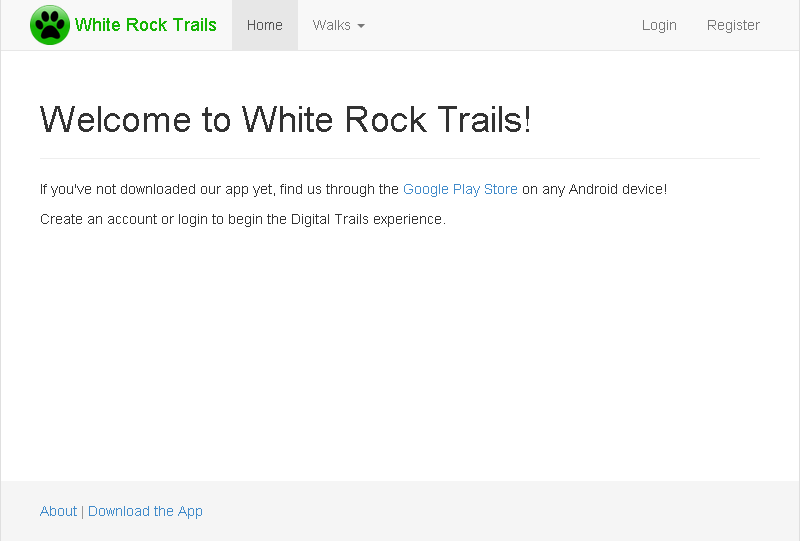
\includegraphics[width=1\linewidth]{./img/webportal/home}
\caption{Home view of the web portal.}
\label{fig:home}
\end{figure}

\paragraph{Responsive View}\mbox{}\\
Figure \ref{fig:home-responsive} demonstrates a responsive view of the web portal. This is the view that users will see when visiting the web portal on mobile devices such as smart phones and tablets. The responsive design minimizes the menu bar which can be expanded by clicking the button shown in the top right of the figure. In addition, web page content reduces in width and elements become stacked allowing for easier scrolling on mobile devices. The responsive design of the web portal is facilitated by the Bootstrap CSS and JavaScript library\cite{milestone2}. The items shown in the list feature navigational links to the associated pages. The \emph{Walks} item expands further child links which navigate to views that are associated with walks.

\begin{figure}[H]
\centering
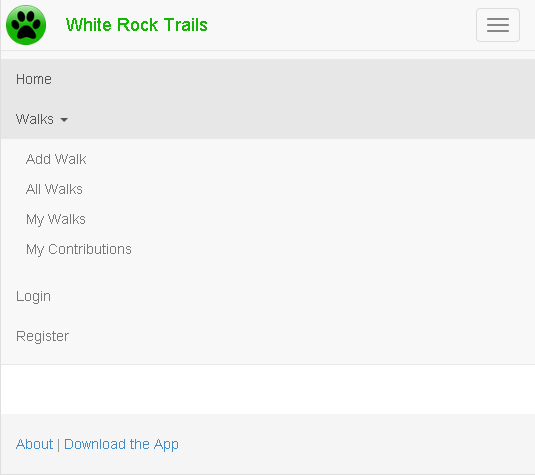
\includegraphics[width=1\linewidth]{./img/webportal/home-responsive}
\caption{Web portal responsive menu view.}
\label{fig:home-responsive}
\end{figure}

\paragraph{Login View}\mbox{}\\
Figure \ref{fig:login} shows the login view that users will see when they click on the \emph{Login} button in the top navigation bar. The login view displays as a modal in front of the web page. This will ensure that users do not have to navigate between pages in order to log in, thus enhancing usability. The login view requires users to input their email address and password followed by clicking the \emph{Login} button. The \emph{Login} button will display a spinner icon whilst the fields are validated to ensure the user is aware that the page is loading. An external validation library is used to validate the fields and display an error or success status. The library uses pre-defined validators to validate the structure of the email address and that the email and password pair is valid when checked against the White Rock Trails API. The validator changes the display of erroneous fields to feature red or green borders and tick or cross icons for invalid and valid fields respectively. A specific error message will also be displayed underneath erroneous fields to inform the reason for the error and allow users to amend it. When users successfully log in, the modal will close and the \emph{Login} and \emph{Registration} buttons shown in the top navigation bar are replaced with the user's full name\cite{milestone2}.

\begin{figure}[H]
\centering
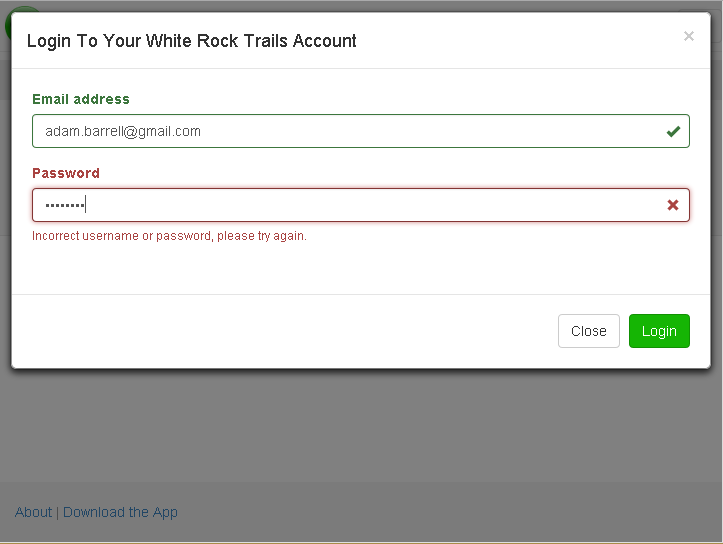
\includegraphics[width=1\linewidth]{./img/webportal/login}
\caption{Web portal login modal demonstrating validation.}
\label{fig:login}
\end{figure}

\paragraph{Registration View}\mbox{}\\
Figure \ref{fig:registration} shows the registration view that users will see when the \emph{Register} button is clicked in the top navigation bar. This view is also implemented as a modal for the same reasons as the login view and to maintain consistency throughout the application. The same validator is also used to validate the registration fields. However, inputs such as \emph{Email Address} and the two password fields require different validators. The former uses a validator that checks whether the provided email address has already been registered by another user. The latter checks whether the two passwords are identical. This will prevent users from registering using a mistyped password and subsequently not being able to log in. Clicking the \emph{Register} button will display a loading spinner inside as described for the login view. When users successfully register, they will be presented with a new confirmation modal instructing them to log in with their new account\cite{milestone2}.

\begin{figure}[H]
\centering
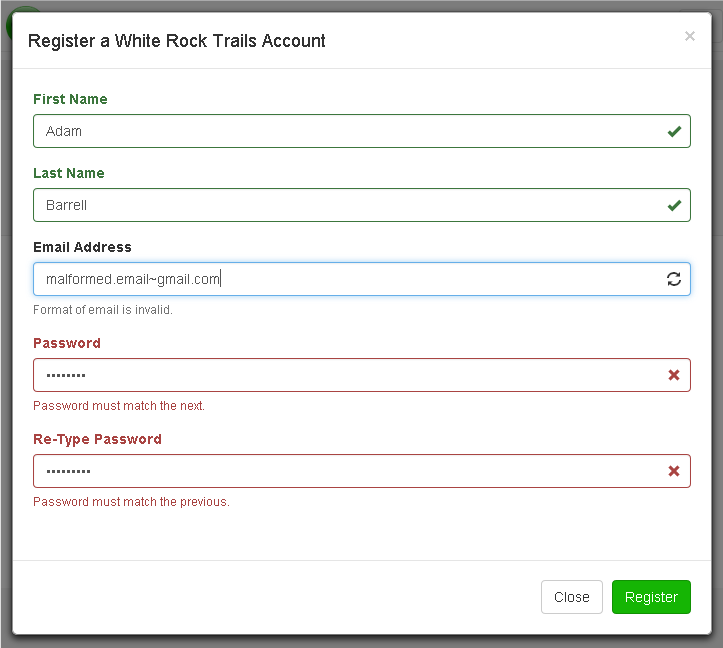
\includegraphics[width=1\linewidth]{./img/webportal/registration}
\caption{Web portal registration modal demonstrating validation.}
\label{fig:registration}
\end{figure}

\paragraph{All Walks View}\mbox{}\\
Figure \ref{fig:all-walks} shows the view users will see when they click on the \emph{Walks} button in the top menu bar and select the \emph{All Walks} option. This view displays a list of tiles, each representing a walk in the database. The background of each tile is an image selected from the collection of each walks way point images. Clicking a tile will navigate the user to a walk information view as presented in Figure \ref{fig:walk-info}\cite{milestone2}. 

Functionality for the \emph{Add Walk} button and search bar have been fully implemented since they were discussed in Milestone 2. Clicking the \emph{Add Walk} button navigates the user to a view where a new walk can be created. Entering text into the search box will perform a full text search of all walks held in the database. The search box also provides instantaneous results such that a request is sent to the server after a set time has expired after a user finishes typing. This allows for much faster and intuitive searching since the user is not required to press a button to execute the search. Finally, pagination has been implemented which allows users to view specific pages of search results that have overflowed the current view. A pagination control is present at the top and bottom of the \emph{All Walks} view for convenience to the user. Users can access specific results pages by clicking the relevant button index. 

\begin{figure}[H]
\centering
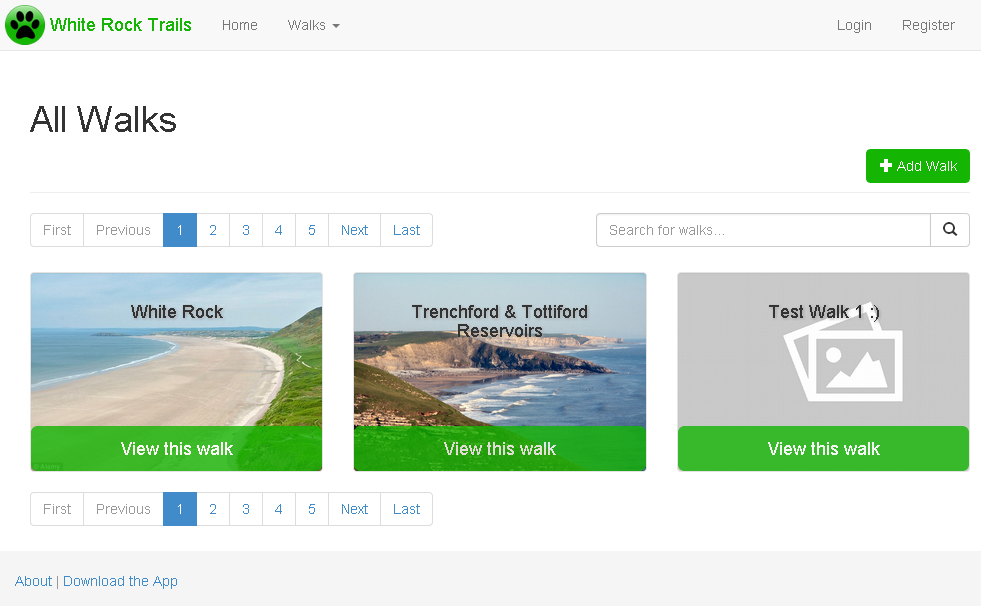
\includegraphics[width=1\linewidth]{./img/webportal/all-walks}
\caption{All walks view of the web portal.}
\label{fig:all-walks}
\end{figure}

\paragraph{Walk Information View}\mbox{}\\
Figure \ref{fig:walk-info} shows the view that a walk owner will see when they click on a walk owned by them from the \emph{All Walks} view. As shown in the figure, walk information will be displayed in this view such a title, description, duration, distance, difficulty rating and author. Navigation tabs above this information allow users to navigate between the \emph{Waypoints}, \emph{Reviews} and \emph{Walk} views. If any waypoint contributions have been submitted to the walk by other users, a \emph{Contributions} tab will appear. The number of pending contributions is also shown adjacent to the tab name. 

The interface also features \emph{Edit} and \emph{Delete} walk buttons which are only visible to the owner of the walk. Clicking the \emph{Edit} button will navigate the user to a view where the walk can be edited, whilst the \emph{delete} will prompt the user to confirm walk deletion. Walk data is asynchronously loaded from the database through the API. The Google Maps API is used to display the map shown in the right of the figure. The Google Maps API allows markers to be placed at specific GPS locations contained within the walk data. The map allows users to scroll and zoom around the walk area to gain an understanding of its location.

\begin{figure}[H]
\centering
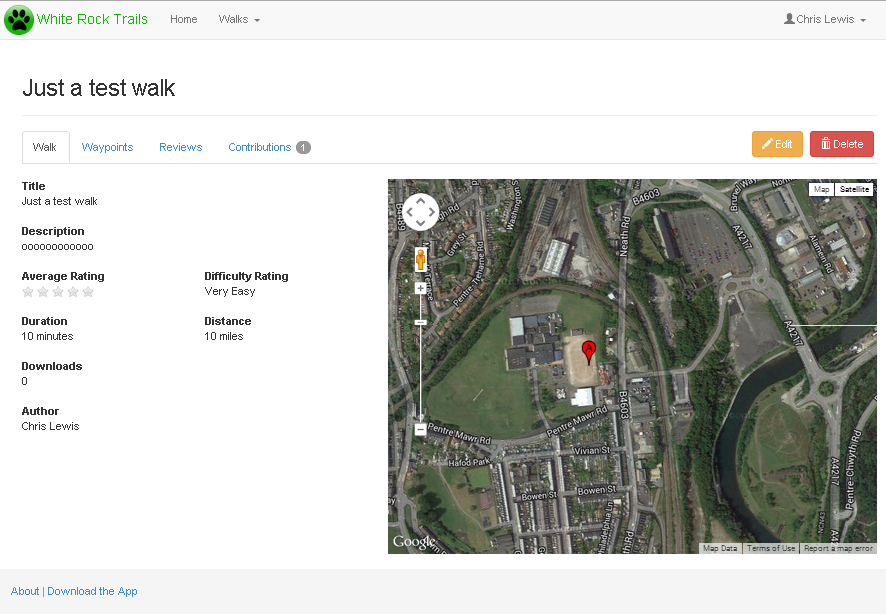
\includegraphics[width=1\linewidth]{./img/webportal/walk-info}
\caption{Walk information view of the web portal.}
\label{fig:walk-info}
\end{figure}

\paragraph{Walk Waypoints View}\mbox{}\\
Figure \ref{fig:walk-waypoints} shows the view that users will see when they click on the \emph{Waypoints} tab of the walk information view. The view shows the list of waypoints that are represented by markers on the map. Markers on the map can be identified by their letter index which references a waypoint shown in the leftmost list list. Clicking a list item or its corresponding map marker will display a modal containing media uploaded to the way point such as images, videos and audio. This feature has been fully implemented since Milestone 2. Finally, a visual fading effect has been applied to the waypoints list where an overflow is present. This indicates to the user that the list panel can be scrolled to display further waypoints.

\begin{figure}[H]
\centering
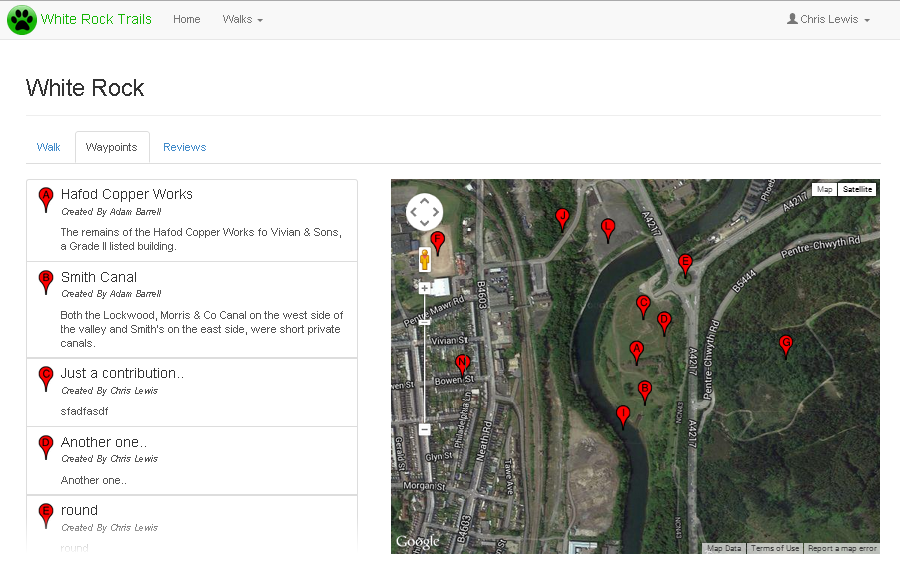
\includegraphics[width=1\linewidth]{./img/webportal/walk-waypoints}
\caption{Walk way points view of the web portal.}
\label{fig:walk-waypoints}
\end{figure}

\paragraph{Walk Reviews View}\mbox{}\\
Figure \ref{fig:walk-reviews} shows the view that users will see when they click the \emph{Reviews} tab from the navigation tabs bar. This view loads user reviews from the walk data and displays them in a list view as shown in the figure. A library called \emph{Raty} was used to generate the star rating system seen below the title of the review. It takes a review rating integer between 1-5 and generates a star representation.

\begin{figure}[H]
\centering
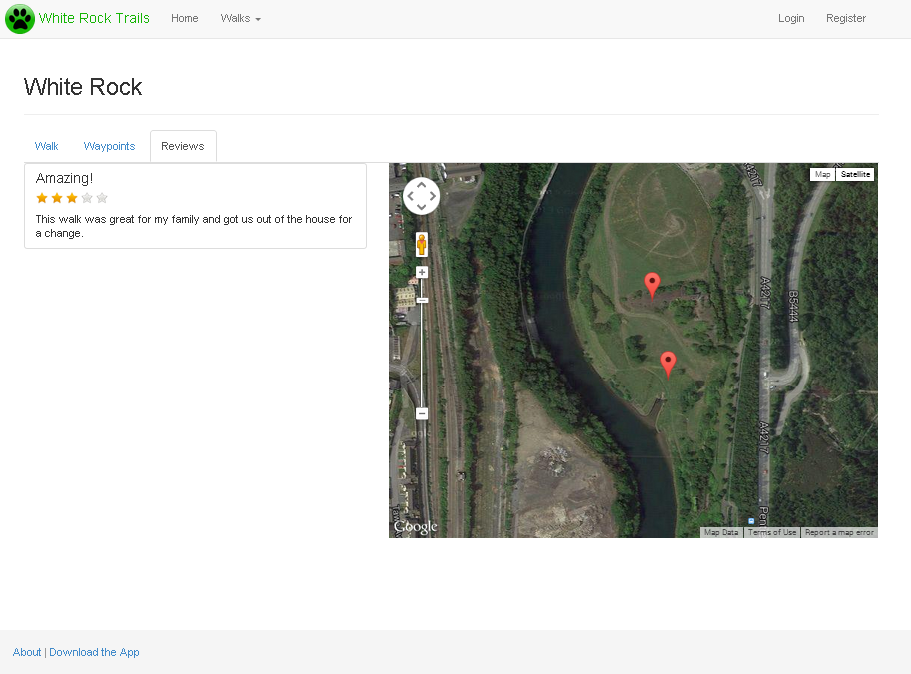
\includegraphics[width=1\linewidth]{./img/webportal/walk-reviews}
\caption{Walk reviews view of the web portal.}
\label{fig:walk-reviews}
\end{figure}

\section{Android Application}
\label{sec:android-design}

\subsection{Rejected Designs}
\label{sec:rejected-designs}

Through-out the course of the project, many design iterations were carried out. As a result, numerous interface designs were modified, while several designs were made redundant for a variety of reasons. This section of the document will analyse rejected designs, highlighting the issues that led to their redundancy. Below is an example of how the interface designs have progressed through several stages of iteration.\\

\textbf{Choose a walk interface} - This example is the walk selection interface ``Saved Walks''. The first iteration took the form of a simple interface design (\ref{fig:view_walk}). Created using Evolus Pencil - An open-source GUI prototyping tool [CITE], the interface included the majority of features set out by Milestone 1 requirements. Here, the user may select from a list of available walks. The main interface window presents the selected walk's name, geological location, description, length (miles) and number of walk waypoints. The interface also included a start button, allowing users to begin the walk in current view.

\begin{figure}[H]
    \centering
    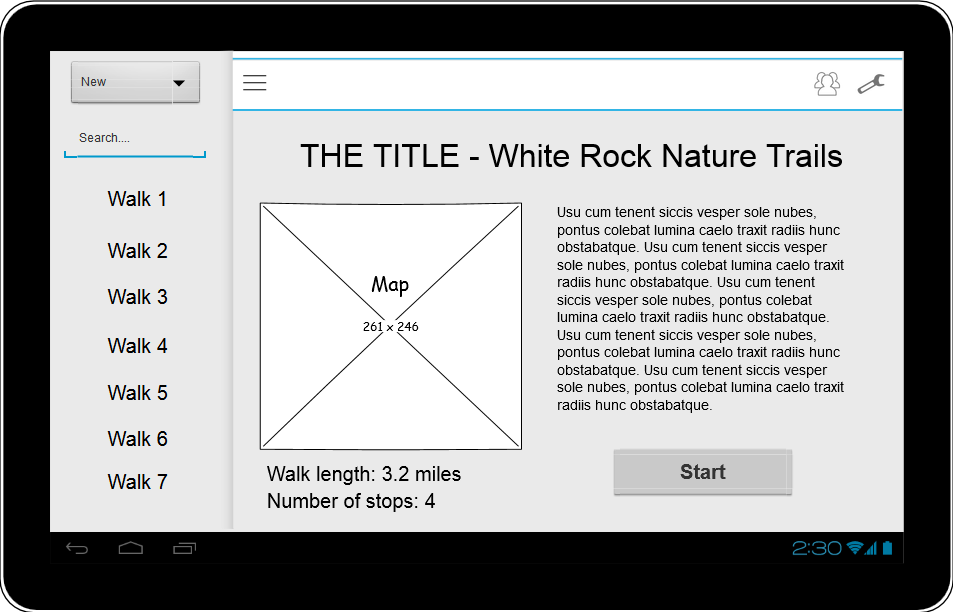
\includegraphics[width=0.8\textwidth]{chris/pencil_choose_walk}
    \caption{Walk selection interface}
    \label{fig:view_walk}
\end{figure}

Based on the initial design, the interface was then created using Eclipse IDE [Cite]. This allowed for a more professional prototype design to be produced, illustrating how the final product may look. It was then possible to carry out improvements on the initial design. The combo-box and search features situated above the list of walks were removed. This was due to the fact they were better suited else where in the application, in a separate search interface. The removal of these two features now allowed for the list of walks to fill the entire side bar fragment. The final stage of this iteration was to add colour to the design. The chosen colour scheme for this iteration was a light shade of green to compliment the application logo. A small amount of shading was applied to the background colour of buttons and other features. 

\begin{figure}[H]
    \centering
    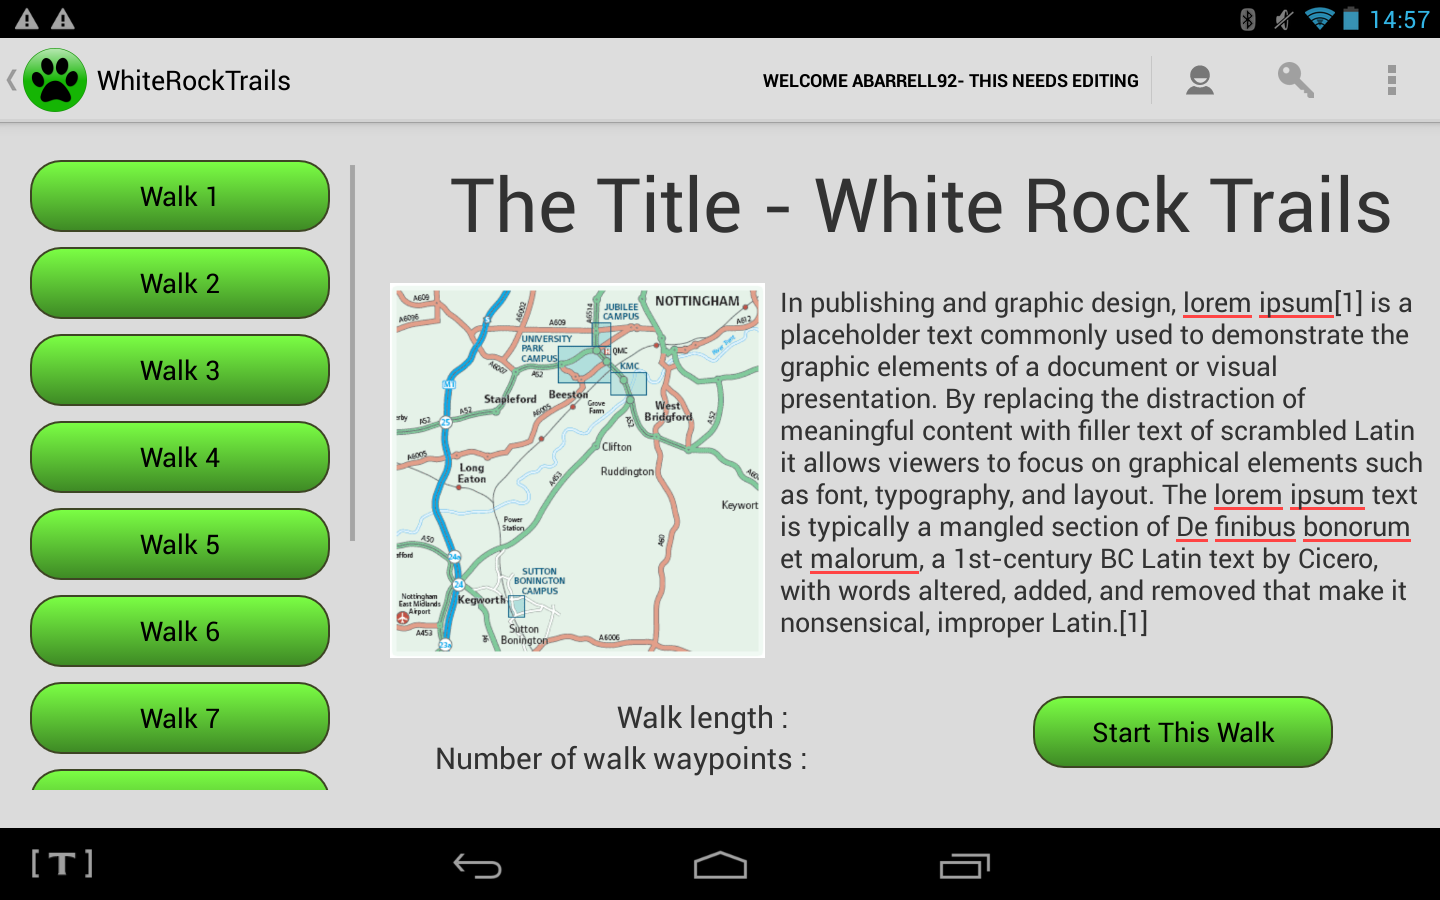
\includegraphics[width=0.8\textwidth]{chris/app_choose_walk}
    \caption{Walk selection interface}
    \label{fig:view_walk}
\end{figure}

ADD FINAL SECTION WHEN APP IS CREATED!!!!!!\\

As previously documented, many interface designs were altered during the iteration stages of development. However, a small number of interface designs were fully rejected and re-designed. Below is a similar example of complete interface re-designs.\\

\textbf{My Walks interface} - The second design iteration saw the ``My Walks'' interface (Figure~\ref{fig:app_my_walks_view}) present each walk create by the user in list form. Each walk included an ID, title, edit and delete button. The user also had the ability to create a new walk from this interface. During evaluation, it was decided that the proposed interface was not suitably designed. It's inappropriate layout meant that the only information available about each walk was in fact its ID and title. Before selecting the edit or delete button, the user may have to view a walk if they were unable to recall by name. The list format also led to a poor use of layout positioning. A vast amount of empty space was visible, especially when using the application on a large tablet.

\begin{figure}[H]
    \centering
    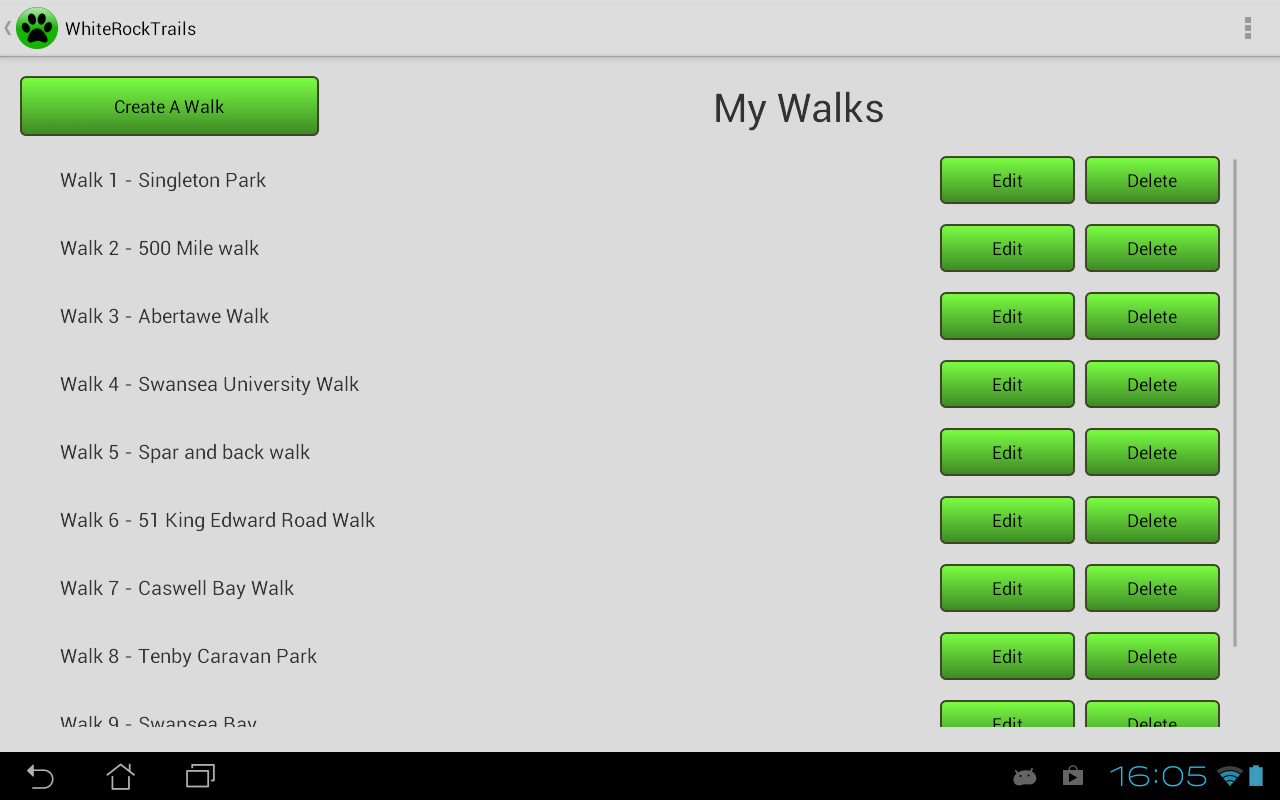
\includegraphics[width=0.8\textwidth]{chris/app_my_walks_view}
    \caption{Walk selection interface}
    \label{fig:app_my_walks_view}
\end{figure}

With the above negative aspects of this design taken into consideration, a new interface design was produced. The interface now presents each walk in a side-bar style list fragment, reading each walk from a database. The edit and delete buttons are included in the main fragment. Additional features to the interface now include the walk's geological location, description, length(miles), number of walk waypoints, difficulty rating and average user rating. Providing this level of information allows users to view a basic summary of each walk created by the user.\\

INSERT THE BETTER IMAGE HERE!!!\\

\subsection{Chosen Design}
\label{sec:chosen-designs}

\section{API}
\label{sec:api-design}

The API is the crucial link between the Website, Application and Database. It was important that the correct design and technology was selected to make that link as seamless as possible. 

\subsection{Possible Designs}
\label{sec:api:rejected-designs} %Phalcon Framework. SOAP API's.
When work started on the API the first descision that needed to be made was on the protocal for the API. There are several popular API protocals including;

\begin{itemize}
\item SOAP
\item REST
\item JSON-RPC 
\item XML-RPC \ldots
\end{itemize}

The most popular two are SOAP and REST. SOAP was originally defined as `Simple Object Access Protocol' and is the sucssesor to XML-RPC (XML Remote Procedure Call). It uses a XML document for its message which is sent over either the HTTP or SMTP application protocals. The XML document which is transmitted with a SOAP request has several parts. The document will start with an `Envelope' which contains all of the data. Inside the `Envelope' there is an optional `Header', a compolsary `Body' which contains request data, and an optional `Fault' which contains any errors which have occured. Listing \ref{lst:soap} shows an example of a SOAP request.

\lstset{language=xml,
keywordstyle=\color{Maroon},
commentstyle=\color{OliveGreen},
showstringspaces=false, tabsize=4, breaklines=true, showspaces=false, stringstyle=\color{Blue}}

\begin{lstlisting}[captionpos=b, caption=An example SOAP request., label=lst:soap, frame=single]
POST /InStock HTTP/1.1
Host: www.example.org
Content-Type: application/soap+xml; charset=utf-8
Content-Length: 299
SOAPAction: "http://www.w3.org/203/05/soap-envelope"
 
<?xml version="1.0"?>
<soap:Envelope xmlns:soap="http://www.w3.org/203/05/soap-envelope">
  <soap:Header>
  </soap:Header>
  <soap:Body>
    <m:GetStockPrice xmlns:m="http://www.example.org/stock">
      <m:StockName>IBM</m:StockName>
    </m:GetStockPrice>
  </soap:Body>
</soap:Envelope>
\end{lstlisting}

REST, on the other hand, is a stateless system which comunicates via URI's, any media (such as JSON or XML) and HTTP Methods. REST stands for Representational State Transfer, which implys a representation of the current state must be transfered to the API with reach request. A REST request to retrive an object can be as simple as \lstinline$GET http:\\example.com\api\users$. The simplicity of REST lends its self to many situations and makes it easy to adapt to specific cases. 

\subsection{Chosen Desgin}
For the API it was decided to harness the REST protocal. The decision was made after analysing both SOAP and REST and the advantages and disadvantages of both. In the end the overly veribose nature of SOAP led to the decision of a REST api.  The ability to use JSON with REST requests was also a deciding factor as this gretly reduced the workload when comunicating with the API from JavaScript. 

\subsection{UML Diagrams}
\label{sec:api:uml}

\subsection{Classes}
\label{sec:api:class}
The API has several `Model' classes to represent the Database tables and the objects that are stored within them. The objects are related through the database and can retrieve the related models through method calls. The relations between the models is shown in Figure \ref{fig:datamodels}, where every model is a possible entry point. Using these models it is possible to, for example, use an `English Walk Description' to return all related 'Waypoint Images'. 

\begin{figure}[H]
    \centering
    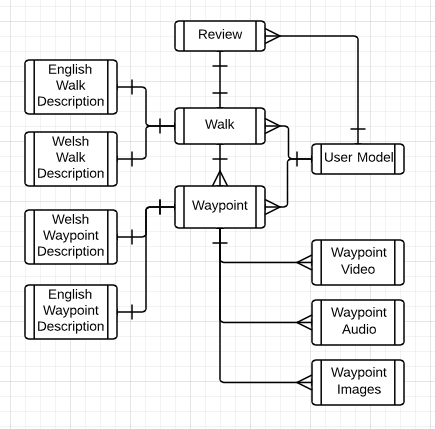
\includegraphics[width=0.5\textwidth]{DataModels}
    \caption{The Data Model and their relations.}
    \label{fig:datamodels}
\end{figure}

The API has several main object collections, which are `Walks', `Waypoints', `Users', `Waypoint Images', `Waypoint Audio', `Waypoint Video', `Walk Reviews' and `Sessions'. Each collection has a specific route in the API which maps to a collection controller. When a route is called a method in the revelvent controller is called. The method is passed a variable called \$app. This contains the requets and response objects. When the controller has completed its work it writes the response to the \$app object and returns to the index file which initally handled the request. If there is no more work to be done the \$app object sends the response. 

\begin{figure}[H]
    \centering
    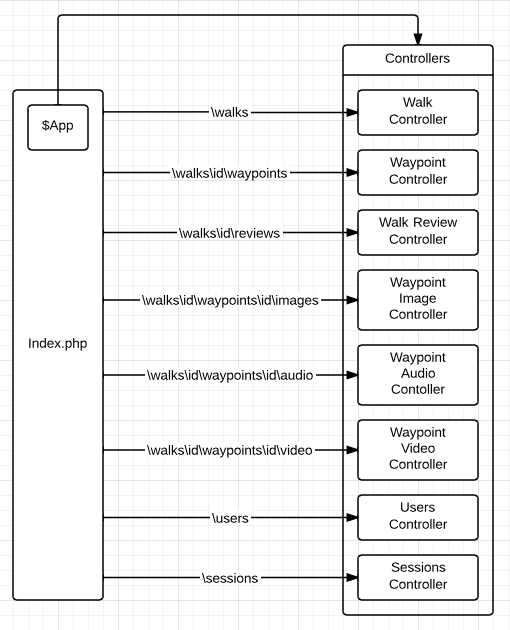
\includegraphics[width=0.5\textwidth]{ControllerRoutes}
    \caption{The connection between routes and controllers.}
    \label{fig:controllerroutes}
\end{figure}

\subsection{Technology Choices}
\label{sec:api:techChoices}

\begin{description}
\item[Paris] - Paris is an ORM (Object Relation Mapper) which provided a layer of abstraction between the database and the API. Rather than writing SQL queries to retrieve an object it makes it possible to use model objects to and methods to retrieve the objects.  
\item[Slim Framework] - The slim framework was chosen as the underlying framework of the API. Slim provides many low-level function which are critical to the production of a reliable API in a small and efficient package. Before it was settled on an alternative framework called Phalcon was trialed, but it proved to be overly complex and overwhelming compared to the relative simplicity of Slim. 
\item[PHP] - This is the language on which Slim runs. It is a popular free and open source web programming langauage. It has great support and is widly used through the world. Alternatives included C\#.NET which is a closed source and closed platform product from Microsoft. Due to the licensing fees and extra costs involved PHP quickly came to light as the best choice. 
\item[Apache] - This is the web server which handles request and responses for the API. It recieves requests and passes them on to the PHP runtime for the API. Apache is the best known and most widely used web server in the world. The alternatives were Nginx and IIS. IIS is limited to Microsfts platforms and Nginx, while well respected, is still an emerging presence in the market. 
\item[Linux] - Linux is the operating system which powers the API server. Linux is free and open source and is the most popular platfrom for operating a server.
\item[JSON] - JavaScript Object Notation (JSON) is a media format which is used to represent JavaScript objects as plain text. It can be used to represent far more than just JavaScript objects however. 
\end{description}

\section{Database}
\label{sec:database-design}
% UML Diagrams
% Descriptions of each entity

\subsection{Rejected Designs}
\label{sec:rejected-designs}

\subsection{Chosen Design}
\label{sec:chosen-designs}

\chapter{Testing}
\label{sec:testing}
\section{Unit Testing}
\label{sec:unit-testint}
\section{Acceptance Testing}
\label{sec:acceptance-testint}

\chapter{User Manual}
\label{sec:user-manual}

\section{API}

\section{Web Portal}

\section{Android Application}

\chapter{Reflective Account}
\label{sec:reflective-account}
\section{Problem Solving}
\label{sec:problem-solving}
\section{Learning Experience}
\label{sec:learning-experience}
\section{Risk Analysis Review}
\label{sec:risk-analysis-review}
\subsection{Anticipated Risks}
\label{sec:anticipated-risks}
\subsection{Un-Anticipated Risks}
\label{sec:unanticipated-risks}
\section{Schedule Review}
\label{sec:schedule-review}
\section{Methodology Review}
\label{sec:methodology-review}
\section{Goals Achieved}
\label{sec:goals-achieved}
\section{Improvements}
\label{sec:improvements}

\chapter*{Summary}
\label{sec:summary}
\addcontentsline{toc}{chapter}{Summary}

%References as subsection
\newpage
\bibliographystyle{plain}
\bibliography{bibliography}

\appendix

\end{document}
